% fig_gfl_gfm_i2ratio.tex
% TR-38: I2 current and 67Q activation vs GFM fraction f_gfm
%
% k_total = 0.20 fixed; f_gfm varies 0→1
% I2_total = k_total * [f_gfm * R2_GFM * 1.5 + (1-f_gfm) * R2_GFL]
% R2_GFL=0.10, R2_GFM=0.40 (transient, I_peak=1.5)
%
% Data points (f_gfm → I2_total):
%  0.00 → 0.20*(0*0.40*1.5 + 1.0*0.10) = 0.020
%  0.20 → 0.20*(0.2*0.60  + 0.8*0.10) = 0.20*(0.12+0.08) = 0.040
%  0.34 → threshold: I2=0.20*(0.34*0.60+0.66*0.10)=0.20*(0.204+0.066)=0.20*0.270=0.054 ≈ I_min_67Q
%  0.50 → 0.20*(0.5*0.60  + 0.5*0.10) = 0.20*(0.30+0.05) = 0.070
%  0.80 → 0.20*(0.8*0.60  + 0.2*0.10) = 0.20*(0.48+0.02) = 0.100
%  1.00 → 0.20*(1.0*0.60  + 0.0*0.10) = 0.20*(0.60)      = 0.120
%
% I_min_67Q = 0.054 (threshold line)

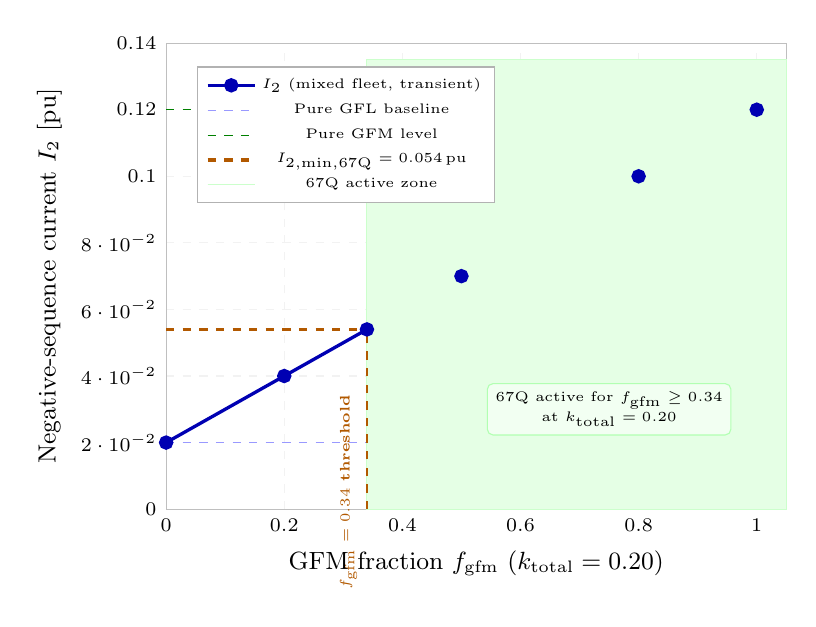
\begin{tikzpicture}
\begin{axis}[
  name         = i2ax,
  width        = 0.78\textwidth,
  height       = 7.5cm,
  xlabel       = {GFM fraction $f_\mathrm{gfm}$ ($k_\mathrm{total}=0.20$)},
  ylabel       = {Negative-sequence current $I_2$ [pu]},
  xlabel style = {font=\small},
  ylabel style = {font=\small},
  xmin=0, xmax=1.05,
  ymin=0, ymax=0.14,
  xtick        = {0,0.2,0.4,0.6,0.8,1.0},
  ytick        = {0,0.02,0.04,0.06,0.08,0.10,0.12,0.14},
  xticklabel style={font=\scriptsize},
  yticklabel style={font=\scriptsize},
  tick style   = {draw=none},
  axis line style={gray!50},
  grid         = major,
  grid style   = {gray!10, dashed},
  legend style = {at={(0.05,0.95)}, anchor=north west, font=\tiny,
                  draw=gray!60, fill=white},
  clip         = false,
]

%% I2 vs f_gfm (mixed fleet, transient)
\addplot[blue!70!black, very thick, mark=*, mark size=2pt]
  coordinates {
    (0.00, 0.020)
    (0.20, 0.040)
    (0.34, 0.054)
    (0.50, 0.070)
    (0.80, 0.100)
    (1.00, 0.120)
  };
\addlegendentry{$I_2$ (mixed fleet, transient)}

%% Pure GFL reference (flat)
\addplot[blue!40, dashed, thin]
  coordinates {(0,0.020) (1.05,0.020)};
\addlegendentry{Pure GFL baseline}

%% Pure GFM reference (flat)
\addplot[green!50!black, dashed, thin]
  coordinates {(0,0.120) (1.05,0.120)};
\addlegendentry{Pure GFM level}

%% 67Q threshold line
\addplot[orange!70!black, very thick, dashed]
  coordinates {(0,0.054) (1.05,0.054)};
\addlegendentry{$I_{2,\min,\mathrm{67Q}}=0.054$\,pu}

%% Shading: 67Q active region (f_gfm >= 0.34)
\addplot[green!20, fill=green!10]
  coordinates {(0.34,0.054) (0.34,0.135) (1.05,0.135) (1.05,0.054)}
  \closedcycle;
\addlegendentry{67Q active zone}

%% Activation marker
\draw[orange!70!black, thick, dashed]
  (axis cs:0.34, 0) -- (axis cs:0.34, 0.054);
\node[orange!70!black, font=\tiny\bfseries, rotate=90, anchor=south]
  at (axis cs:0.34, 0.005)
  {$f_\mathrm{gfm}=0.34$ threshold};

%% Annotation box
\node[draw=green!30, fill=green!5, rounded corners=2pt,
      font=\tiny, inner sep=3pt, align=center]
  at (axis cs:0.75, 0.030)
  {67Q active for $f_\mathrm{gfm}\geq0.34$\\
   at $k_\mathrm{total}=0.20$};

\end{axis}
\end{tikzpicture}
